\chapter{Differentiable Contact Dynamics}

We present Dojo, a differentiable physics engine for robotics that prioritizes stable simulation, accurate contact physics, and differentiability with respect to states, actions, and system parameters. Dojo achieves stable simulation at low sample rates and conserves energy and momentum by employing a variational integrator. A nonlinear complementarity problem, with second-order cones for friction, models hard contact and is reliably solved using a custom primal-dual interior-point method. Special properties of the interior-point method are exploited using implicit differentiation to efficiently compute smooth gradients that provide useful information through contact events. We demonstrate Dojo's unique ability to simulate hard contact while providing smooth, analytic gradients with a number of examples, including trajectory optimization, policy optimization, and system identification.

\vspace*{\fill}

\noindent Dojo: A Differentiable Physics Engine for Robotics. Taylor A. Howell$^*$, Simon Le Cleac'h$^*$, Zico Kolter, Mac Schwager, and Zachary Manchester. arXiv 2203.00806. 2022.

\pagebreak

\section{Introduction}
The last decade has seen immense resources devoted to network architectures, optimization algorithms, and the construction of large datasets by the learning community. These efforts have been leveraged to make impressive advances in robotics including: dexterous manipulation \cite{andrychowicz2020learning,akkaya2019solving}, quadrupedal locomotion \cite{lee2020learning, kumar2021rma}, and pixels-to-torques control \cite{levine2018learning}. In contrast, there has been comparatively little work on the lowest level of the robotics stack: the \textit{physics engine}. We argue that deficiencies in current widely used physics engines form a key bottleneck that must be overcome to enable future advancements in robotics. 

Physics engines that simulate rigid-body dynamics with contact are utilized for trajectory optimization, reinforcement learning, system identification, and dataset generation for domains ranging from locomotion to manipulation. To be of practical value in real-world applications and overcome the sim-to-real gap an engine should provide stable simulation, accurately emulate a robot's dynamics, and ideally, be differentiable to enable use of efficient gradient-based optimization methods.

In recent years, a number of physics engines \cite{drake, freeman2021brax, werling2021fast, geilinger2020add, hu2019difftaichi, heiden2020neuralsim} have been developed and utilized for robotics. In this work, we address key deficiencies of these tools including: high sample rates required for stable simulation that exacerbate the vanishing/exploding gradient problem and substantially increase sample complexities for rollout-based optimization methods, interpenetration of rigid bodies (e.g., a robot foot sinking through the floor) or creep (e.g., objects that should be at rest incorrectly sliding), and lack of informative gradients  through contact events (e.g., subgradients resulting from naïve differentiation of non-smooth dynamics) or expensive gradients that require a large number of calls to the engine (e.g., finite-difference or stochastic-sampling schemes).

The Dojo physics engine is designed from the ground up to enable better and easier optimization for motion planning, control, reinforcement learning, system identification, and high-quality dataset generation. By taking a physics- and optimization-first approach to physics-engine design, we significantly advance the state of the art in \textit{stable simulation}, \textit{accurate contact physics}, and \textit{differentiability} for robot simulation. Key attributes of Dojo include: 
\begin{itemize}
	\item Variational integration for stable simulation that is not sensitive to time step size
	\item A nonlinear complementarity problem (NCP) model for accurate contact dynamics
	\item A custom primal-dual interior-point method for reliably solving the NCP 
	\item Smooth, analytic gradients that provide useful information through contact events
\end{itemize}

In the remainder of this chapter, we first provide an overview of related state-of-the-art physics engines in Section \ref{dojo_related_work}. Next, we present Dojo, and its key features, in Section \ref{dojo}. Simulation, planning, policy optimization, and system identification examples are presented in Section \ref{dojo_results}. Finally, we discuss Dojo's limitations in Section \ref{dojo_limitations} and provide closing remarks in Section \ref{dojo_future_work}.

\section{Related Work} \label{dojo_related_work}

This section provides an overview of physics engines that are commonly used in robotics. Table \ref{dojo_engine_comparison} summarizes the features of these tools and compares them to Dojo.

Many physics engines being developed and used in practice today were not designed for real-world robotics applications, and it is common for these tools to prioritize the \textit{appearance} of realism over actual physical accuracy. Additionally, many of these physics engines were designed primarily for graphics and animation applications where fast simulation rates are prioritized and general-purpose numerical-optimization routines that do not natively support key elements from robotics domains, like cone constraints or quaternions, are commonplace. In this section, we provide background on a collection of popular engines, including: discussion of physical fidelity, underlying optimization routines, and ability to return gradients.

In the learning community, \emph{MuJoCo}~\cite{todorov2012mujoco} has become a standard for benchmarking reinforcement learning algorithms using the OpenAI Gym environments~\cite{brockman2016openai}.
MuJoCo utilizes minimal-coordinates representations and employs both semi-implicit Euler and explicit fourth-order Runge-Kutta integrators to simulate multi-body systems. These integrators often require small time steps, particularly for systems experiencing contact, and typically sample rates of hundreds to thousands of Hertz are required for stable simulation, which a mature and efficient implementation is able to achieve much faster than real-time rates. However, the high simulation rates can prove a challenge for control tasks like reinforcement learning settings where vanishing or exploding gradients are exacerbated over long horizons with many time steps.

Impact and friction are modeled using a smooth, convex contact model \cite{todorov2014convex}. While this approach reliably computes contact forces, it introduces artificial damping, allowing the system to experience unphysical interpenetration and forces at a distance (i.e., while not in contact) and the default friction model introduces additional artifacts like velocity drift during sliding. Additionally, achieving good simulation behavior often requires system-specific tuning of multiple solver parameters. Further, the ``soft" contact model is computed using a \textit{primal} optimization method, meaning that as parameters are set to produce ``hard,'' or more realistic contact, the underlying optimization problem becomes increasingly ill-conditioned and difficult to solve. As a result, it is often not possible to eliminate unphysical artifacts from the simulation and produce realistic results. Finally, analytical gradients are not provided by the engine, requiring finite-difference schemes.

\emph{Drake \cite{drake}} was designed for robotics applications and its contact dynamics primarily rely on the classic time-stepping contact model that solves a linear complementarity problem (LCP) at each time step \cite{stewart1996implicit}. To satisfy the LCP problem formulation, a number of approximations are made to the dynamics and contact model, including the use of an approximate friction cone. To ensure stability of the simulation, small time steps are used where linearizations of the dynamics are valid, but importantly, the engine can achieve accurate hard contact. General-purpose LCP solvers that are typically used rely on a pivoting method like Lemke's algorithm \cite{cottle2009linear}. Randomized smoothing has been proposed as a method for returning gradients through contact \cite{suh2022bundled} with this model. Higher-fidelity models are available for patch contacts \cite{elandt2019pressure}, but they are computationally more expensive, requiring sophisticated higher-order implicit integrators.

The popular robotics simulator \emph{Gazebo} \cite{koenig2004design} can utilize several different physics engines to simulate multi-body contact dynamics; Bullet \cite{heiden2020neuralsim} and DART \cite{lee2018dart} are common choices. Similar to Drake, these engines model hard contact dynamics with a LCP formulation. Automatic differentiation tools have also been utilized to compute gradients \cite{heiden2020neuralsim}. However, because of the discontinuous nature of contact dynamics, this approach will sometimes return sub-gradients, which do not provide useful information through contact events. Heuristics have been proposed to enumerate contact modes in order to select informative sub-gradients \cite{werling2021fast}. However, this approach scales poorly with the number of mode switches.

Engines designed for hardware accelerators (e.g., GPUs), including \emph{Brax} \cite{freeman2021brax} and \emph{PhysX} \cite{physx2022engine}, utilize simplified contact models that are amenable to low-precision data types (e.g., Float32). The benefit is massive parallel computation. However, these engines often require system-specific tuning to achieve stable simulation and the results are typically lower-fidelity.

Building on previous work \cite{brudigam2021linear}, Dojo utilizes the open-source maximal-coordinates dynamics library \texttt{ConstrainedDynamics.jl} and efficient graph-based linear-system solver \texttt{GraphBasedSystems.jl} to compute smooth dynamics. However, unlike this prior work, Dojo has an improved contact model, specifically with regard to friction and its representation in the graph structure. Additionally, Dojo implements an efficient and reliable differentiable interior-point solver for complementarity problems.

The properties and characteristics of these existing engines are summarized in Table \ref{dojo_engine_comparison}. We find that none of the existing engines prioritize two of the most important attributes for robotics: physical accuracy and useful differentiability. This motivates our development of a new physics engine for robotics applications.

\begin{table}[H]
	\centering
	\caption[Comparison of physics engines used for robotics]{Comparison of physics engines used for robotics.}
	\small
	\begin{tabular}{c c c c c c c}
		\toprule
		\textbf{Engine} & \textbf{Integrator} & \textbf{State} & \textbf{Contact} & \textbf{Solver} & \textbf{Gradients} \\
		\toprule
		MuJoCo \cite{todorov2012mujoco} & RK4 & minimal & soft & Newton & finite-difference \\
		Drake \cite{drake} & implicit Euler & minimal & soft/hard & LCP & randomized-smoothing\\
		Bullet \cite{coumans2019} & implicit Euler & minimal & soft/hard & LCP & sub-gradient \\
		DART \cite{lee2018dart} & implicit Euler & minimal & hard & LCP & sub-gradient\\
		PhysX \cite{physx2022engine} & explicit & minimal & soft & iterative & finite-difference \\
		Brax \cite{freeman2021brax} & explicit & maximal & soft & iterative & sub-gradient\\
		\hline
		\textbf{Dojo} & variational & maximal & hard & NCP & implicit gradient \\
		\toprule
	\end{tabular}
	\label{dojo_engine_comparison}
\end{table}
%===============================================================================

\section{Dojo} \label{dojo}

We now introduce Dojo's contact dynamics model and custom interior-point solver. This section presents the key algorithms and subroutines, including: variational integrators, the contact model, a differentiable primal-dual interior-point solver, and the computation of smooth gradients. An open-source implementation of the engine is provided.

\subsection{Maximal-coordinates representation} 
Most multi-body physics engines utilize minimal- or joint-coordinates representations for dynamics because of the small number of states and convenience of implementation. This results in small, but dense systems of linear equations. In contrast, maximal-coordinates explicitly represent the position, orientation, and velocities of each body in a multi-body system. This produces large, sparse systems of linear equations that can be efficiently solved, including in the contact setting. We provide an overview, largely based on prior work \cite{brudigam2020linear}, of this representation. 

A single rigid body is defined by its mass and inertia, and has a configuration, $x = (p, q) \in \mathbf{X} = \mathbf{R}^3 \times \mathbf{H}$, comprising a position $p$ and unit quaternion $q$, where $\mathbf{H}$ is the space of four-dimensional unit quaternions. We define the implicit discrete-time dynamics $F : \mathbf{X} \times \mathbf{X} \times \mathbf{X} \rightarrow \mathbf{R}^{6}$ as: 
\begin{equation}
	F(x_{-}, x, x_{+}) = 0, \label{dojo_implicit_dynamics}
\end{equation}
where we indicate the previous and next time steps with minus ($-$) and plus ($+$) subscripts, respectively, and the current time step without decoration.
A variational integrator is employed to simulate the next state of the system and has desirable energy and momentum conservation properties \cite{marsden2001discrete}. Linear and angular velocities are handled implicitly via finite-difference approximations.

For a multi-body system with bodies $a$ and $b$ connected via a joint---common types include: revolute, prismatic, and spherical---we introduce a constraint, $k : \mathbf{X} \times \mathbf{X} \rightarrow \mathbf{R}^{l}$, that couples the two bodies: 
\begin{equation} 
	k^{ab}(x^{a}_{+}, x^{b}_{+}) = 0. 
\end{equation} 
An impulse, $j \in \mathbf{R}^l$, where $l$ is equal to the six degrees-of-freedom of an unconstrained body minus the joint's number of degrees-of-freedom, acts on both bodies to satisfy the constraint. The implicit integrator for the multi-body system has the form,
\begin{equation} 
	\begin{bmatrix} 
		F^{a}(x^{a}_{-}, x^{a}, x^{a}_{+}) + K^{a}(x^{a}, x^{b})^T j^{ab} \\ 
		F^{b}(x^{b}_{-}, x^{b}, x^{b}_{+}) + K^{b}(x^{a}, x^{b})^T j^{ab} \\ 
		k^{ab}(x^{a}_{+}, x^{b}_{+})
	\end{bmatrix} = 0, \label{dojo_max_2body}
\end{equation}
where $K: \mathbf{X} \times \mathbf{X} \rightarrow \mathbf{R}^{l \times 6}$ is a mapping from the joint to the maximal-coordinates space and is related to the Jacobian of the joint constraint.

We can generalize  \eqref{dojo_max_2body} to include additional bodies and joints. For a system with $N$ bodies and $M$ joints we define a maximal-coordinates configuration $z = (x^{(1)}, \dots, x^{(N)}) \in \mathbf{Z}$ and joint impulse $j = (j^{(1)}, \dots, j^{(M)}) \in \mathbf{J}$. We define the implicit discrete-time dynamics of the maximal-coordinates system as: 
\begin{equation} 
	F(z_{-}, z, z_{+}, j) = 0, \label{dojo_max_implicit_dynamics}
\end{equation}
where $F: \mathbf{Z} \times \mathbf{Z} \times \mathbf{Z} \times \mathbf{J} \rightarrow \mathbf{R}^{6N}$. In order to simulate the system we find $z_{+}$ and $j$ that satisfy \eqref{dojo_max_implicit_dynamics} for a provided $z_{-}$ and $z$ using Newton's method. 

By exploiting the mechanism's structure, we can efficiently perform root finding on \eqref{dojo_max_implicit_dynamics} (see \cite{brudigam2020linear} for additional details). This structure is manifest as a graph of the mechanism, where each body and joint is considered a node, and joints have edges connecting bodies (Fig. \ref{dojo_graph_structure}). Because the mechanism structure is known \textit{a priori}, a permutation matrix can be precomputed and used to perform efficient sparse linear algebra during simulation. For instance, in the case where the joint constraints form a system without loops, the resulting sparse system can be solved in linear time with respect to the number of links.

\begin{figure}[H]
	\centering
	\includegraphics[width=0.75\columnwidth]{dojo/graph.tikz}
	\caption[Graph structure for maximal-coordinates state representation]{Graph structure for maximal-coordinates system with 4 bodies, 3 joints, and 3 points of contact.}
	\label{dojo_graph_structure}
\end{figure}

\subsection{Variational integrator}
We use a specialized implicit integrator that preserves energy and momentum, natively handles quaternions, and alleviates spurious artifacts that commonly arise from contact interactions. 

Dojo utilizes a maximal-coordinates state representation \cite{brudigam2020linear}. Each body has linear:
\begin{equation} 
	m (p_{+} - 2 p + p_{-}) / h - h m g - A(p)^T j - h f = 0, \label{dojo_linear_integrator}
\end{equation}
and rotational: 
\begin{equation}
	\sqrt{1 - \psi_+^T \psi_+} J \psi_+ + \psi_+ \times J \psi_+ - \sqrt{1 - \psi^T \psi} J \psi + \psi \times J \psi - B(q)^T j - h^2 \tau / 2 = 0,
	\label{dojo_rotational_integrator}
\end{equation}
dynamics specified by mass $m \in \mathbf{R}_{++}$, inertia $J \in \mathbf{S}_{++}^3$, gravity $g \in \mathbf{R}^3$, and time step $h \in \mathbf{R}_{++}$. Equations (\ref{dojo_linear_integrator}, \ref{dojo_rotational_integrator}) are essentially second-order centered-finite-difference approximations of Newton's second law and Euler's equation for the rotational dynamics where $q_+ = q \cdot (\sqrt{1 - \psi_+^T \psi_+}, \psi_+)$ is recovered from a three-parameter representation $\psi \in \mathbf{R}^3$ \cite{manchester2016quaternion}, respectively. Joint impulses $j \in \mathbf{J}$ have linear $A : \mathbf{R}^3 \rightarrow \mathbf{R}^{\mbox{dim}(\mathbf{J}) \times 3}$ and rotational $B : \mathbf{H} \rightarrow \mathbf{R}^{\mbox{dim}(\mathbf{J}) \times 3}$ mappings into the dynamics. The configuration of a body $z^{(i)} = (p^{(i)}, q^{(i)}) \in \mathbf{R}^3 \times \mathbf{H}$ comprises a position and orientation represented as a quaternion. Forces and torques $f, \tau \in \mathbf{R}^3$ can be applied to the bodies.

Both \eqref{dojo_linear_integrator} and \eqref{dojo_rotational_integrator} are derived by approximating Hamilton's Principle of Least-Action using a simple midpoint scheme \cite{marsden2001discrete,manchester2020variational}. This approach produces \emph{variational} integrators that automatically conserve momentum and energy \cite{marsden2001discrete}.

\subsection{Rigid-body dynamics with contact}
Impact and friction behaviors are modeled, along with the system's dynamics, as a complementarity problem. This model simulates hard contact without requiring system-specific solver tuning. Additionally, contacts between a system and the environment are treated as a single graph node connected to a rigid body (Fig \ref{dojo_graph_structure}). As a result, the engine retains efficient linear-time complexity for open-chain mechanical systems.

Dojo uses the classic impact model (\ref{intro_sdf}-\ref{intro_impact_inequality}) and in the following section we present a Coulomb friction model that utilizes an exact nonlinear friction cone.

\paragraph{Second-order friction cone.}
In contrast to the LCP formulation, we utilize the optimality conditions of \eqref{intro_mdp} in a form amenable to a primal-dual interior-point solver. The associated cone program is,
\begin{equation}
	\begin{array}{ll}
		\underset{\beta}{\mbox{minimize}} & v^T \beta_{(2:3)}\\
		\mbox{subject to} & \beta_{(1)} = \mu \gamma, \\
		& \|\beta_{(2:3)}\|_2 \leq \beta_{(1)},\\
	\end{array} \label{dojo_mdp_socp}
\end{equation}
where subscripts indicate vector indices.
The relaxed optimality conditions for (\ref{dojo_mdp_socp}) in interior-point form are: 
\begin{align}
	v - \eta_{(2:3)} &= 0, \\
	\beta_{(1)} - \mu \gamma &= 0, \\
	\beta \circ \eta &=  \kappa \mathbf{e}, \\
	\|\beta_{(2:3)}\|_2 \leq \beta_{(1)}, \, \|\eta_{(2:3)}\|_2 &\leq \eta_{(1)}, 
	\label{socp_mdp_constraints}
\end{align}
with dual variable $\eta \in \mathbf{R}^3$ associated with the second-order-cone constraints, and central-path parameter, $\kappa \in \mathbf{R}_{+}$. The benefits of this model are increased physical fidelity and fewer optimization variables, without substantial increase in computational cost.

\paragraph{Complementarity problem.}
Rigid-body dynamics with a single contact (this formulation extends to multiple contacts) is simulated using a time-stepping scheme that solves the feasibility problem,
\begin{align}
	\label{dojo_ncp}
	{\mbox{find}} \quad & z_{+}, j, \gamma, \beta, \eta\\
	\mbox{subject to} \quad & F(z_{-}, z, z_{+}, j, \lambda, u) = 0, \notag \\
	& v_c(z, z_{+}) - \eta_{(2:3)} = 0, \notag \\
	& \beta_{(1)} - \mu \gamma = 0, \notag\\
	& \gamma \cdot \phi(z_{+}) = \kappa, \notag \\
	& \beta \circ \eta = \kappa \mathbf{e}, \notag \\
	& \gamma, \phi(z_{+}) \geq 0, \, \|\beta_{(2:3)}\|_2 \leq \beta_{(1)}, \, \|\eta_{(2:3)}\|_2 \leq \eta_{(1)}, \notag
\end{align}
with actions $u = (f^{(1)}, \tau^{(1)}, \dots, f^{(N)}, \tau^{(N)}) \in \mathbf{U}$, and contact impulses $\lambda = (\beta_{(2:3)}, \gamma) \in \mathbf{\Lambda}$. The system's smooth dynamics $F : \mathbf{Z} \times \mathbf{Z} \times \mathbf{Z} \times \mathbf{J} \times \mathbf{\Lambda} \times \mathbf{U} \rightarrow \mathbf{R}^{6N}$ comprise linear and rotational dynamics (\ref{dojo_linear_integrator}-\ref{dojo_rotational_integrator}) for each body \cite{brudigam2020linear}. The central-path parameter $\kappa \in \mathbf{R}_{+}$ and target $\mathbf{e}$ \cite{vandenberghe2010cvxopt} are utilized by the interior-point solver in the following section. 

Solving the feasibility problem finds a maximal-coordinates state representation. In many applications it is desirable to utilize a minimal-coordinates representation (e.g., direct trajectory optimization where algorithm complexity scales with the state dimension). Dojo includes functionality to analytically convert between representations, as well as formulate and apply the appropriate chain rule in order to differentiate through a representation transformation.

To simulate a system forward in time one step, given a control input and state comprising the previous and current configurations, solutions to a sequence of barriers problems \eqref{dojo_ncp} are found with $\kappa \rightarrow 0$. The central-path parameter has a physical interpretation as being the softness of the contact model. A value $\kappa = 0$ corresponds to exact ``hard" or inelastic contact, whereas a relaxed value produces soft contact where contact forces can occur at a distance. The primal-dual interior-point solver described in the next section adaptively decreases this parameter in order to efficiently and reliably converge to hard contact solutions. In practice, the engine is set to converge to small values for simulation in order to simulate accurate physics. Intermediate solutions (i.e., $\kappa \neq 0$) are cached and later utilized to compute smooth gradients in order to provide useful information through contact events.

\subsection{Solver} 

To efficiently and reliably satisfy \eqref{dojo_ncp}, we developed a custom primal-dual interior-point solver for NCPs with support for cone constraints and quaternions. The algorithm is largely based upon Mehrotra's predictor-corrector algorithm \cite{mehrotra1992implementation, nocedal2006numerical}, while implementing non-Euclidean optimization techniques to handle quaternions \cite{jackson2021planning} and borrowing features from CVXOPT \cite{vandenberghe2010cvxopt} to handle cones. 

The primary advantages of this algorithm are the correction to the classic Newton step, which can greatly reduce the iterations required by the solver (often halving the total number of iterations), and feedback on the problem's central-path parameter that helps avoid premature ill-conditioning and adaptively drives the complementarity violation to zero in order to reliably simulate hard contact.

\paragraph{Problem.}
The solver aims to satisfy instantiations of the following problem:
\begin{equation}
	\begin{array}{ll}
		\underset{}{\mbox{find}} & a, b, c \\
		\mbox{subject to} & E(a, b, c; \theta) = 0, \\
		& b \circ c = \kappa \mathbf{e}, \\
		& b, c \in \mathcal{K},
	\end{array} \label{dojo_ncp_abstract}
\end{equation}
with decision variables $a \in \mathbf{R}^{n_{a}}$ and $b, c \in \mathbf{R}^{n_{b}}$, equality-constraint set $E : \mathbf{R}^{n_{a}} \times \mathbf{R}^{n_{b}} \times \mathbf{R}^{n_{b}} \times \mathbf{R}^{n_{\theta}} \rightarrow \mathbf{R}^{n_a + n_{b}}$, problem data $\theta \in \mathbf{R}^{n_{\theta}}$; and where $\mathcal{K}$ is the Cartesian product of positive-orthant and second-order cones \cite{boyd2004convex}. 

Interior-point methods aim to satisfy a sequence of relaxed problems with $\kappa > 0$ and $\kappa \rightarrow 0$ in order to reliably converge to a solution of the original problem (i.e., $\kappa = 0$). This continuation approach helps avoid premature ill-conditioning and is the basis for numerous convex and non-convex interior-point solvers \cite{nocedal2006numerical}.

The LCP formulation is a special-case instantiation \eqref{dojo_ncp_abstract} where the constraint set is affine in the decision variables, the cone is the positive orthant. Most general-purpose solvers for LCPs rely on active-set methods that strictly enforce $\kappa = 0$ at each iteration.

\paragraph{Residual and Jacobians.}
The interior-point solver aims to find a fixed point for the residual:
\begin{align}
	r(w; \theta, \kappa) &= \begin{bmatrix}
		E(w;\theta) \\
		b^{(1)} \circ c^{(1)} - \kappa \mathbf{1}\\
		\vdots \\
		b^{(n_{\mathcal{K}})} \circ c^{(n_{\mathcal{K}})} - \kappa \mathbf{e}\\
	\end{bmatrix}, \label{dojo_residual}
\end{align}
while respecting the cone constraints.
The Jacobian of this residual with respect to the decision variables,
\begin{equation}
	R(w; \theta) = \partial r(w; \theta, \cdot) / \partial w, \label{dojo_var_jacobian}
\end{equation}
is used to compute a search direction. For convenience, we denote $w = (a, b, c)$. After a solution $w^*(\theta, \kappa)$ is found, the Jacobian of the residual with respect to the problem data,
\begin{equation}
	D(w; \theta) = \partial r(w; \theta, \cdot) / \partial \theta , \label{dojo_data_jacobian}
\end{equation}
is used to compute the sensitivity of the solution. These Jacobians are not explicitly dependent on the central-path parameter.

The non-Euclidean properties of quaternion variables are handled with modifications to these Jacobians \eqref{dojo_var_jacobian} and \eqref{dojo_data_jacobian} by right multiplying each with a matrix $H$ containing attitude Jacobians \cite{jackson2021planning} corresponding to the quaternions in $x$ and $\theta$, respectively: 
\begin{align}
	\bar{R}(w; \theta) &= R(w; \theta) H_{R}(w), \\ 
	\bar{D}(w; \theta) &= D(w; \theta) H_{D}(\theta).
\end{align}
Euclidean variables have corresponding identity blocks. This modification accounts for the implicit unit-norm constraint on each quaternion variable and improves the convergence behavior of the solver.

\paragraph{Analytical line search for cones.}
To ensure the cone variables strictly satisfy their constraints, a cone line search is performed for a candidate search direction. For the update:
\begin{align}
	y \leftarrow y + \alpha \Delta,
\end{align}
with step size $\alpha$ and search direction $\Delta$, the solver finds the largest $\alpha \in [0, 1]$ such that $y + \alpha \Delta \in \mathcal{K}$. The step-size is computed analytically for the positive orthant:
\begin{align}
	\alpha = \mbox{min} \left(1,  \underset{k | \Delta_{(k)} < 0}{\mbox{max}} \Big \{ -\frac{y_{(k)}}{\Delta_{(k)}} \Big \} \right), 
	\label{dojo_alpha_ort}
\end{align}
and second-order cone:
\begin{align}
	\nu &= y_{(1)}^2 - y_{(2:k)}^T y_{(2:k)}, \\
	\zeta &= y_{(1)} \Delta_{(1)} - y_{(2:k)}^T \Delta_{(2:k)}, \\
	\rho_{(1)} &= \frac{\zeta}{\nu}, \\
	\rho_{(2:k)} &= \frac{\Delta_{(2:k)}}{\sqrt{\nu}} - \frac{\zeta / \sqrt{\nu} + \Delta_{(1)}}{y_{(1)} / \sqrt{\nu} + 1} \frac{y_{(2:k)}}{\nu}, \\
	\alpha &= \begin{cases}
		\mbox{min} \left( 1, \frac{1}{\|\rho_{(2:k)}\|_2 - \rho_{(1)}} \right), \quad \|\rho_{(2:k)}\|_2 > \rho_{(1)}, \\
		1, \quad \mbox{otherwise}.
	\end{cases}
	\label{dojo_alpha_soc}
\end{align}
The line search over all individual cones is summarized in Algorithm \ref{dojo_cls_algo}.

\begin{algorithm}[H]
	\caption{Analytical Line Search For Cones}\label{dojo_cls_algo}
	\begin{algorithmic}[1]
		\Procedure{ConeLineSearch}{$w, \Delta, \tau^{\mbox{ort}}, \tau^{\mbox{soc}}$}
		\State $\alpha_y^{\mbox{ort}} \gets \alpha(y^{(1)}, \tau^{\mbox{ort}} \Delta^{y^{(1)}}) $ \Comment{Eq. \ref{dojo_alpha_ort}}
		\State $\alpha_z^{\mbox{ort}} \gets \alpha(z^{(1)}, \tau^{\mbox{ort}} \Delta^{z^{(1)}}) $ \Comment{Eq. \ref{dojo_alpha_ort}}
		
		\State $\alpha_y^{\mbox{soc}} \gets \underset{i \in \{2, \dots, n \}}{\mbox{min}} \alpha(y^{(i)}, \tau^{\mbox{soc}} \Delta^{y^{(i)}})$ \Comment{Eq. \ref{dojo_alpha_soc}}
		\State $\alpha_z^{\mbox{soc}} \gets \underset{i \in \{2, \dots, n \}}{\mbox{min}} \alpha(z^{(i)}, \tau^{\mbox{soc}} \Delta^{z^{(i)}})$ \Comment{Eq. \ref{dojo_alpha_soc}}
		\State \textbf{Return} $\mbox{min}(\alpha_y^{\mbox{ort}}, \alpha_z^{\mbox{ort}}, \alpha_y^{\mbox{soc}}, \alpha_z^{\mbox{soc}})$
		\EndProcedure
	\end{algorithmic}
\end{algorithm}

\paragraph{Candidate update.} 
The variables are partitioned: $a = (a^{(1)}, \dots, a^{(p)})$, where $i = 1$ are Euclidean variables and $i = 2, \dots, p$ are each quaternion variables; and $b = (b^{(1)}, \dots, b^{(n)})$, $c = (c^{(1)}, \dots, c^{(n)})$, where $j = 1$ is the positive-orthant and the remaining $j = 2, \dots, n$ are second-order cones.
For a given search direction, updates for Euclidean and quaternion variables are performed. The Euclidean variables in $a$ use a standard update: 
\begin{equation} 
	a^{(1)} \leftarrow a^{(1)} + \alpha \Delta^{(1)}, \label{dojo_standard_update}
\end{equation}
For each quaternion variable, the search direction exists in the space tangent to the unit-quaternion hypersphere and is 3-dimensional. The corresponding update for $i = 2, \dots, p$ is: 
\begin{equation}
	a^{(i)} \leftarrow L(a^{(i)}) \varphi(\alpha \Delta^{(i)}), \label{dojo_quaternion_update}
\end{equation}
where $L : \mathbf{H} \rightarrow \mathbf{R}^{4 \times 4}$ is a matrix representing a left-quaternion matrix multiplication, and $\varphi : \mathbf{R}^3 \rightarrow \mathbf{H}$ is a mapping to a unit quaternion. The standard update is used for the remaining decision variables $b$ and $c$.

\paragraph{Violation metrics.}
Two metrics are used to measure progress: 
The constraint violation, 
\begin{align}
	r_{\mbox{vio}} = \| r(w; \theta) \|_{\infty},
	\label{dojo_r_vio}
\end{align}
and complementarity violation,
\begin{align}
	\kappa_{\mbox{vio}} = \underset{i}{\mbox{max}} \{\| b^{(i)} \circ c^{(i)} \|_{\infty}\}.
	\label{dojo_kappa_vio}
\end{align}
The problem \eqref{dojo_ncp_abstract} is considered solved when $r_{\mbox{vio}} < r_{\mbox{tol}}$ and $\kappa_{\mbox{vio}} < \kappa_{\mbox{tol}}$.

\paragraph{Centering.}
The solver adaptively relaxes \eqref{dojo_ncp_abstract} by computing the centering parameters $\mu$ and $\sigma$. These values provide an estimate of the cone-constraint violation and determine the value of the central-path parameter that a correction step will aim to satisfy. These values rely on the degree of the cone \cite{vandenberghe2010cvxopt}:
\begin{equation}
	\mbox{\textbf{deg}}(\mathcal{K}) = \sum_{i=1}^{n_{\mathcal{K}}} \mbox{\textbf{deg}}(\mathcal{K}^{(i)}) = \mbox{\textbf{dim}}(\mathcal{K}^{(1)}) + n_{\mathcal{K}} - 1 \label{dojo_centering_0},
\end{equation}
the complementarity violations:
\begin{equation}
	\mu = \frac{1}{\mbox{\textbf{deg}}(\mathcal{K})} \sum_{i = 1}^{n_{\mathcal{K}}} (b^{(i)})^T c^{(i)}, \label{dojo_centering_1}
\end{equation}
and affine complementarity violations: 
\begin{equation}
	\mu^{\mbox{aff}} = \frac{1}{\mbox{\textbf{deg}}(\mathcal{K})} \sum_{i = 1}^{n_{\mathcal{K}}} (b^{(i)} + \alpha \Delta^{b^{(i)}})^T (c^{(i)} + \alpha \Delta^{c^{(i)}}), \label{dojo_centering_2}
\end{equation}
as well as their ratio:
\begin{equation}
	\sigma = \mbox{min}\left(1, \mbox{max} \left(0, \mu^{\mbox{aff}} / \mu \right) \right)^3,
	\label{dojo_centering_3}
\end{equation}
As the algorithm makes progress, it aims to reduce these violations.

\paragraph{Algorithm.}
The interior-point algorithm used to solve \eqref{dojo_ncp_abstract} is summarized in Algorithm \ref{dojo_interiorpoint}. Additional tolerances $\tau \in [0.9, 1]$ are used to improve numerical reliability of the solver. The algorithm parameters include $\tau^{\mbox{soc}}_{\mbox{max}}$ to prevent the iterates from reaching the boundaries of the cones too rapidly during the solve, $\tau_{\mbox{min}}$ to ensure we are aiming at sufficiently large steps, and $\beta$ is the decay rate of the step size $\alpha$ during the line search. In practice, $r_{\mbox{tol}}$ and $\kappa_{\mbox{tol}}$ are the only parameters the user might want to tune.

Finally, the algorithm outputs a solution $w^*(\theta, \kappa)$ that satisfies the solver tolerance levels and, optionally, the implicit gradients of the solution with respect to the problem parameters $\theta$.

For an instance of problem \eqref{dojo_ncp_abstract}, the algorithm is provided problem data and an initial point, which is projected to ensure that the cone variables are initially feasible with some margin. Next, an affine search direction (i.e., predictor) is computed that aims for zero complementarity violation. Using this direction, a cone line search is performed followed by a centering step that computes a target relaxation for the computation of the corrector search direction. A second cone line search is then performed for this new search direction. A subsequent line search is performed until either the constraint or complementarity violation is reduced. The current point is then updated, a new affine search direction is computed, and the procedure repeats until the violations satisfy the solver tolerances. 

\begin{algorithm}[H]
	\caption{Primal-Dual Interior-Point Solver} \label{dojo_interiorpoint}
	\begin{algorithmic}[1]
		\Procedure{Optimize}{$a_0, b_0, c_0, \theta, \mathcal{K}$}
		\State \textbf{Parameters}: $\tau^{\mbox{soc}}_{\mbox{max}} = 0.99, \tau_{\mbox{min}} = 0.95$
		\State $r_{\mbox{tol}} = 10^{-5}, \kappa_{\mbox{tol}} = 10^{-5}, \beta = 0.5$
		\State \textbf{Initialize}: $a = a_0, b = b_0 \in \mathcal{K}, c = c_0 \in \mathcal{K}$
		\State $r_{\mbox{vio}}, \kappa_{\mbox{vio}} \gets \Call{Violation}{w}$ \Comment{(\ref{dojo_r_vio}, \ref{dojo_kappa_vio})}
		
		\State \textbf{Until} $r_{\mbox{vio}} < r_{\mbox{tol}}$ \textbf{and} $\kappa_{\mbox{vio}} < \kappa_{\mbox{tol}}$ \textbf{do} 
		\State \indent \hspace{-4mm} $\Delta^{\mbox{aff}} \gets  - \bar{R}^{-1}(w; \theta) r(w; \theta, 0)$
		\State \indent \hspace{-4mm} $\alpha^{\mbox{aff}} \gets \Call{ConeSearch}{w, \Delta^{\mbox{aff}}, 1, 1}$
		
		\State \indent \hspace{-4mm} $\mu, \sigma \gets  \Call{Center}{b, c, \alpha^{\mbox{aff}}, \Delta^{\mbox{aff}}} $ \Comment{(\ref{dojo_centering_0}-\ref{dojo_centering_3})}
		
		\State \indent \hspace{-4mm} $\kappa \gets \mbox{max} (\sigma \mu, \kappa_{\mbox{tol}} / 5)$
		\State \indent \hspace{-4mm} $\Delta \gets  - \bar{R}^{-1}(w; \theta) r(w; \theta, \kappa)$
		\State \indent \hspace{-4mm} $\tau^{\mbox{ort}} \gets \mbox{max}(\tau_{\mbox{min}}, 1 - \mbox{max}(r_{\mbox{vio}}, \kappa_{\mbox{vio}})^2)$ 
		\State \indent \hspace{-4mm} $\tau^{\mbox{soc}} \gets \mbox{min}(\tau^{\mbox{soc}}_{\mbox{max}}, \tau^{\mbox{ort}})$ 
		\State \indent \hspace{-4mm} $\alpha \gets \Call{ConeSearch}{w, \Delta, \tau^{\mbox{ort}}, \tau^{\mbox{soc}}}$
		\State \indent \hspace{-4mm} $c^*_{\mbox{vio}}, \kappa^*_{\mbox{vio}} \gets r_{\mbox{vio}}, \kappa_{\mbox{vio}}$
		\State \indent \hspace{-4mm} \indent \hspace{-4mm} $\hat{w} \gets \Call{Update}{w, \Delta, \alpha}$ \Comment{(\ref{dojo_standard_update}, \ref{dojo_quaternion_update})}
		\State \indent \hspace{-4mm} \indent \hspace{-4mm} $r_{\mbox{vio}}, \kappa_{\mbox{vio}} \gets \Call{Violation}{\hat{w}}$ \Comment{(\ref{dojo_r_vio}, \ref{dojo_kappa_vio})}
		\State \indent \hspace{-4mm} \textbf{Until} $r_{\mbox{vio}} \leq c^*_{\mbox{vio}}$ \textbf{or} $\kappa_{\mbox{vio}} \leq \kappa^*_{\mbox{vio}}$ \textbf{do}
		\State \indent \hspace{-4mm} \indent \hspace{-4mm} $\alpha \leftarrow \beta \alpha$
		\State \indent \hspace{-4mm} \indent \hspace{-4mm} $\hat{w} \gets \Call{Update}{w, \Delta, \alpha}$ \Comment{(\ref{dojo_standard_update}, \ref{dojo_quaternion_update})}
		\State \indent \hspace{-4mm} \indent \hspace{-4mm} $r_{\mbox{vio}}, \kappa_{\mbox{vio}} \gets \Call{Violation}{\hat{w}}$ \Comment{(\ref{dojo_r_vio}, \ref{dojo_kappa_vio})}
		\State \indent \hspace{-4mm} \textbf{end}
		
		\State \indent \hspace{-4mm} $w \leftarrow \hat{w}$
		\State \textbf{end}
		
		\State $\partial w^* / \partial \theta \gets - \bar{R}^{-1}(w^*; \theta) \bar{D}(w^*; \theta)$ \Comment{(\ref{intro_solution_sensitivity})}
		\State \textbf{Return} $w, \partial w^* / \partial \theta$ 
		\EndProcedure
	\end{algorithmic}
\end{algorithm}

\subsection{Gradients} 

Interior-point methods solve non-smooth problems by optimizing a  smooth barrier sub-problems, where the degree of smoothing is parameterized by the central-path parameter $\kappa$. In the contact setting, we employ this same technique to return gradients that are informative through contact events. Intermediate solutions, $w^*(\theta, \kappa > 0)$, are differentiated using the implicit-function theorem \eqref{intro_solution_sensitivity} to compute smooth \textit{implicit gradients}. In practice, we find that these gradients greatly improve the performance of gradient-based optimization methods, consistent with the long history of interior-point methods. Dojo's gradients are compared with sub-gradients and randomized smoothing in Fig. \ref{dojo_gradient_compare}. 

\begin{figure}[H]
	\centering
	\includegraphics{dojo/gradients.tikz}
	\caption[Gradient comparison for Dojo implicit gradients and gradient bundles]{Gradient comparison between subgradients (black), randomized-smoothing gradients \cite{suh2022bundled} (orange, blue) and Dojo's analytic gradients (magenta). The dynamics for a box in the $XY$ plane that is resting on a flat surface and displaced an amount $\Delta$ by a force $f$ (top left). Randomized smoothing gradients (right column) are computed using $500$ samples with varying covariances $\Sigma$. Dojo's gradients (middle column) are computed for different values of central-path parameter $\kappa$. Compared to Dojo, the randomized smoothing method produces noisy derivatives that are many times more expensive to compute.}
	\label{dojo_gradient_compare}
\end{figure}

A wall-clock-time comparison of these gradients and sampled gradients is provided in Table \ref{dojo_compute_ratios}, demonstrating that implicit gradients are more than an order of magnitude faster to compute.

\begin{table}[H]
	\centering
	\caption[Compute ratio for Dojo gradient computation and simulation steps with maximal-coordinates representation]{Compute-time ratio between Dojo's gradient and simulation-step evaluations for maximal-coordinates representation. We compute the engine's implicit gradient with respect to the initial configuration, velocity and control input. For a large system like Atlas, using a finite-difference (FD) scheme to evaluate the dynamics Jacobian in maximal coordinates would require at least 400 simulation-step evaluations. Alternatively, Dojo computes this Jacobian at the cost of approximately 4 simulation-step evaluations: a potential $100$ times speedup on a single thread.}
	\begin{tabular}{c c c c c c}
		\toprule
		\textbf{} & \textbf{Atlas} & \textbf{Humanoid} & \textbf{Quadruped} & \textbf{Ant} & \textbf{Half-Cheetah} \\
		\toprule
		Dojo & 3.7 & 4.9 & 2.5 & 2.3 & 1.2 \\
		FD & 472.6 & 194.7 & 170.3 & 197.0 & 94.8 \\
		\toprule
	\end{tabular}
	\label{dojo_compute_ratios}
\end{table}

The problem data for each simulation step include: the previous and current configurations, control input, and additional terms like the time step, friction coefficients, and parameters of each body. 

\subsection{Implementation}

An open-source implementation, \texttt{Dojo.jl}, written in Julia, is available and a Python interface, \texttt{dojopy}, is also included. These tools, and the experiment, are available at:
\begin{center}
\url{https://github.com/dojo-sim}
\end{center}

\section{Results} \label{dojo_results}
Dojo's capabilities are highlighted through a collection of examples, including: simulating physical phenomena, gradient-based planning with trajectory optimization, policy-optimization, and real-to-sim system identification. The current implementation supports point, sphere, and capsule collisions with flat surfaces. All of the experiments were performed with an Intel Core i9-10885H CPU and 32GB of memory.

\subsection{Simulation}

The simulation accuracy of Dojo and MuJoCo is compared in a number of illustrative  scenarios.

\paragraph{Impact comparison.} 

The Atlas humanoid is simulated dropping on to a flat surface (Fig. \ref{dojo_atlas_drop}). The system comprises 31 bodies, resulting in 403 maximal-coordinates states, and has 36 actuated degrees-of-freedom. Each foot has four contact points. The current implementation of Dojo simulates this system in real time at 65 Hz. 

\begin{figure}[H]
	\centering
	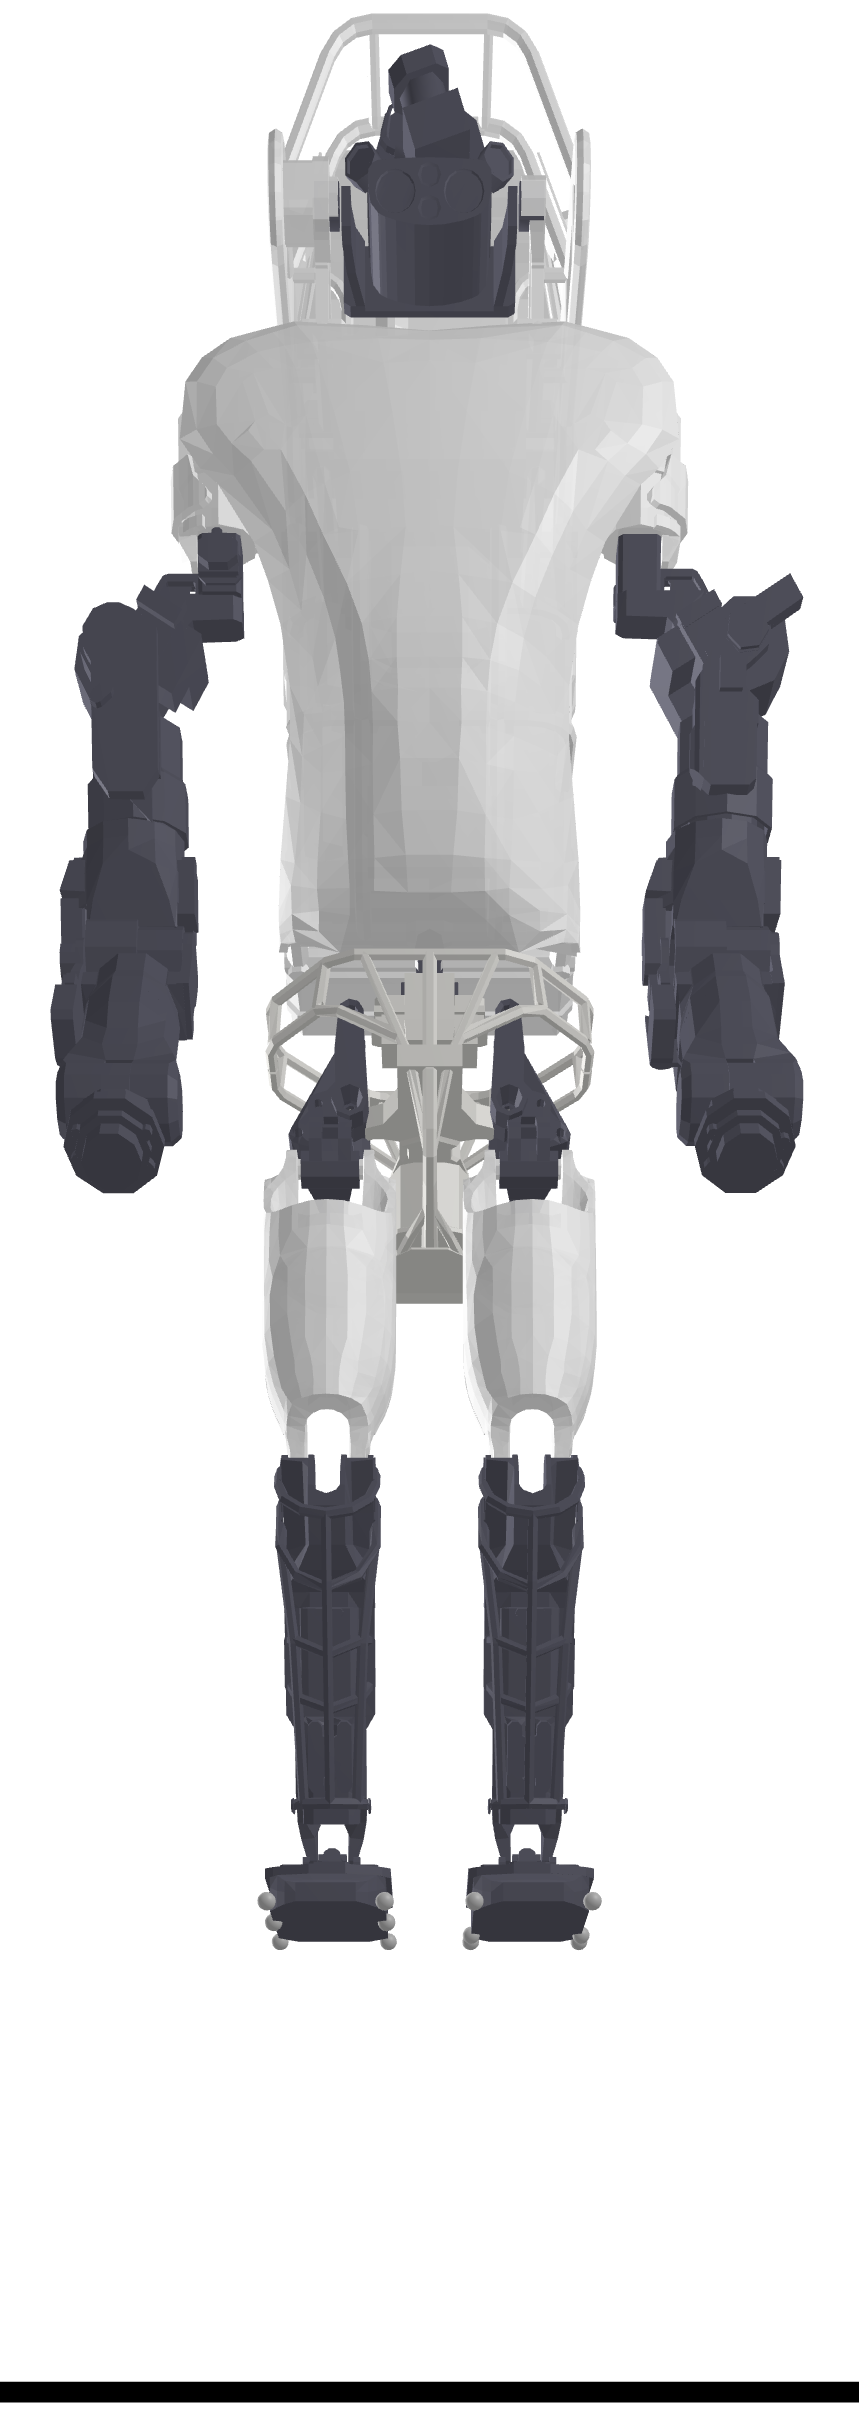
\includegraphics[height=5.0cm]{dojo/atlas1.png} 
	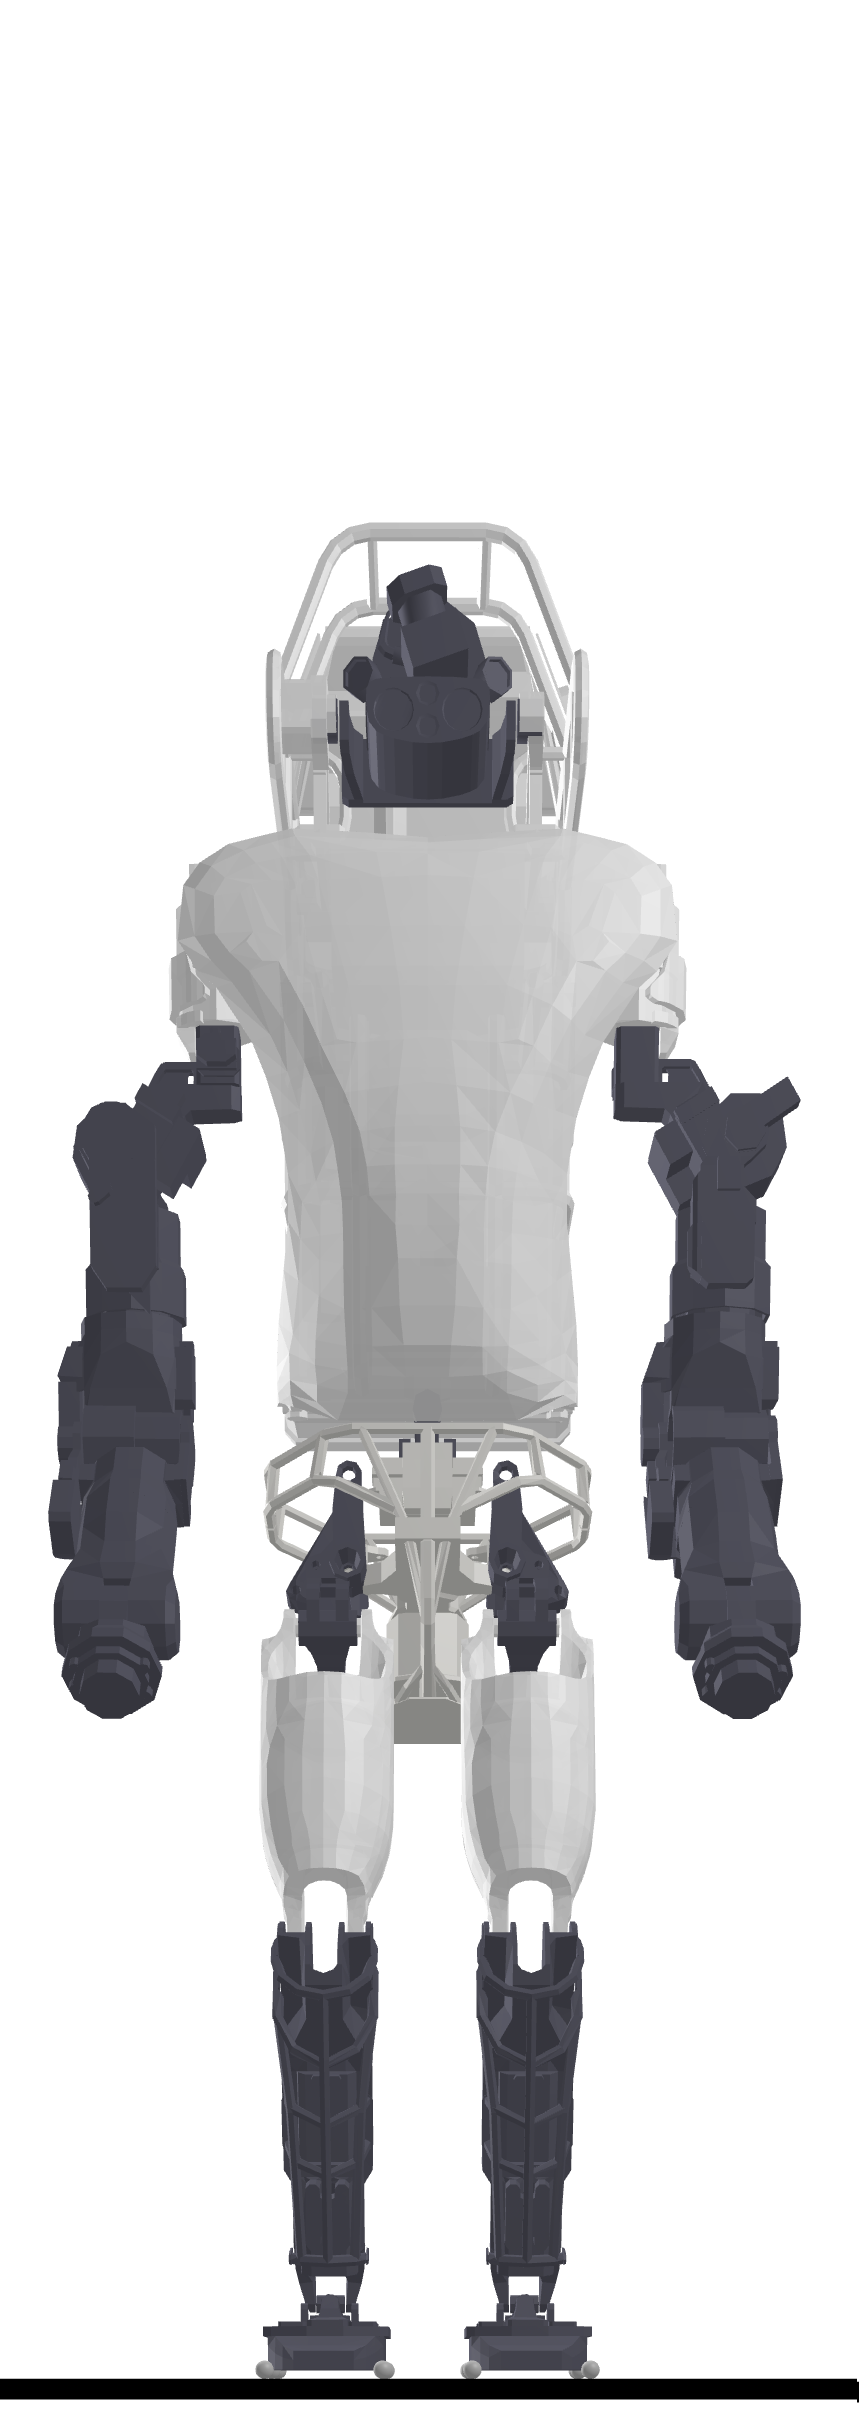
\includegraphics[height=5.0cm]{dojo/atlas2.png}
	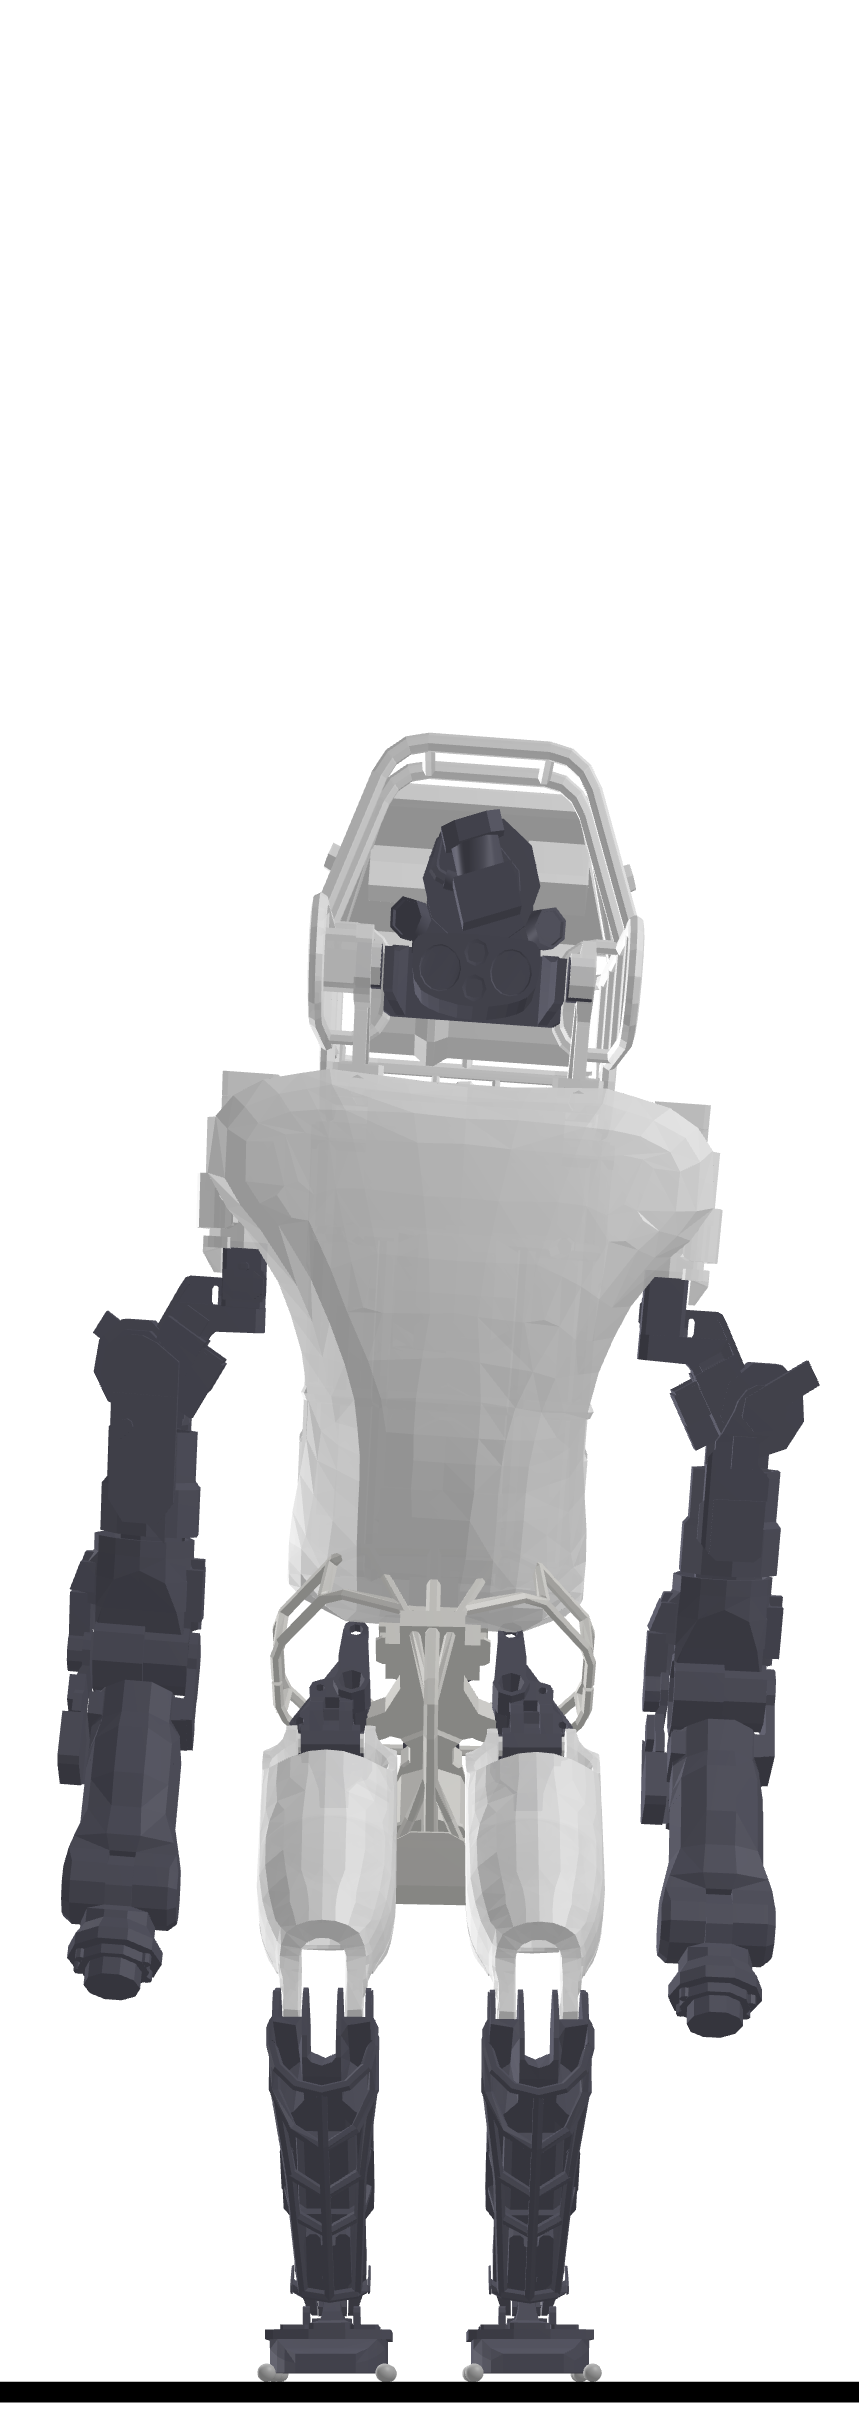
\includegraphics[height=5.0cm]{dojo/atlas3.png}
	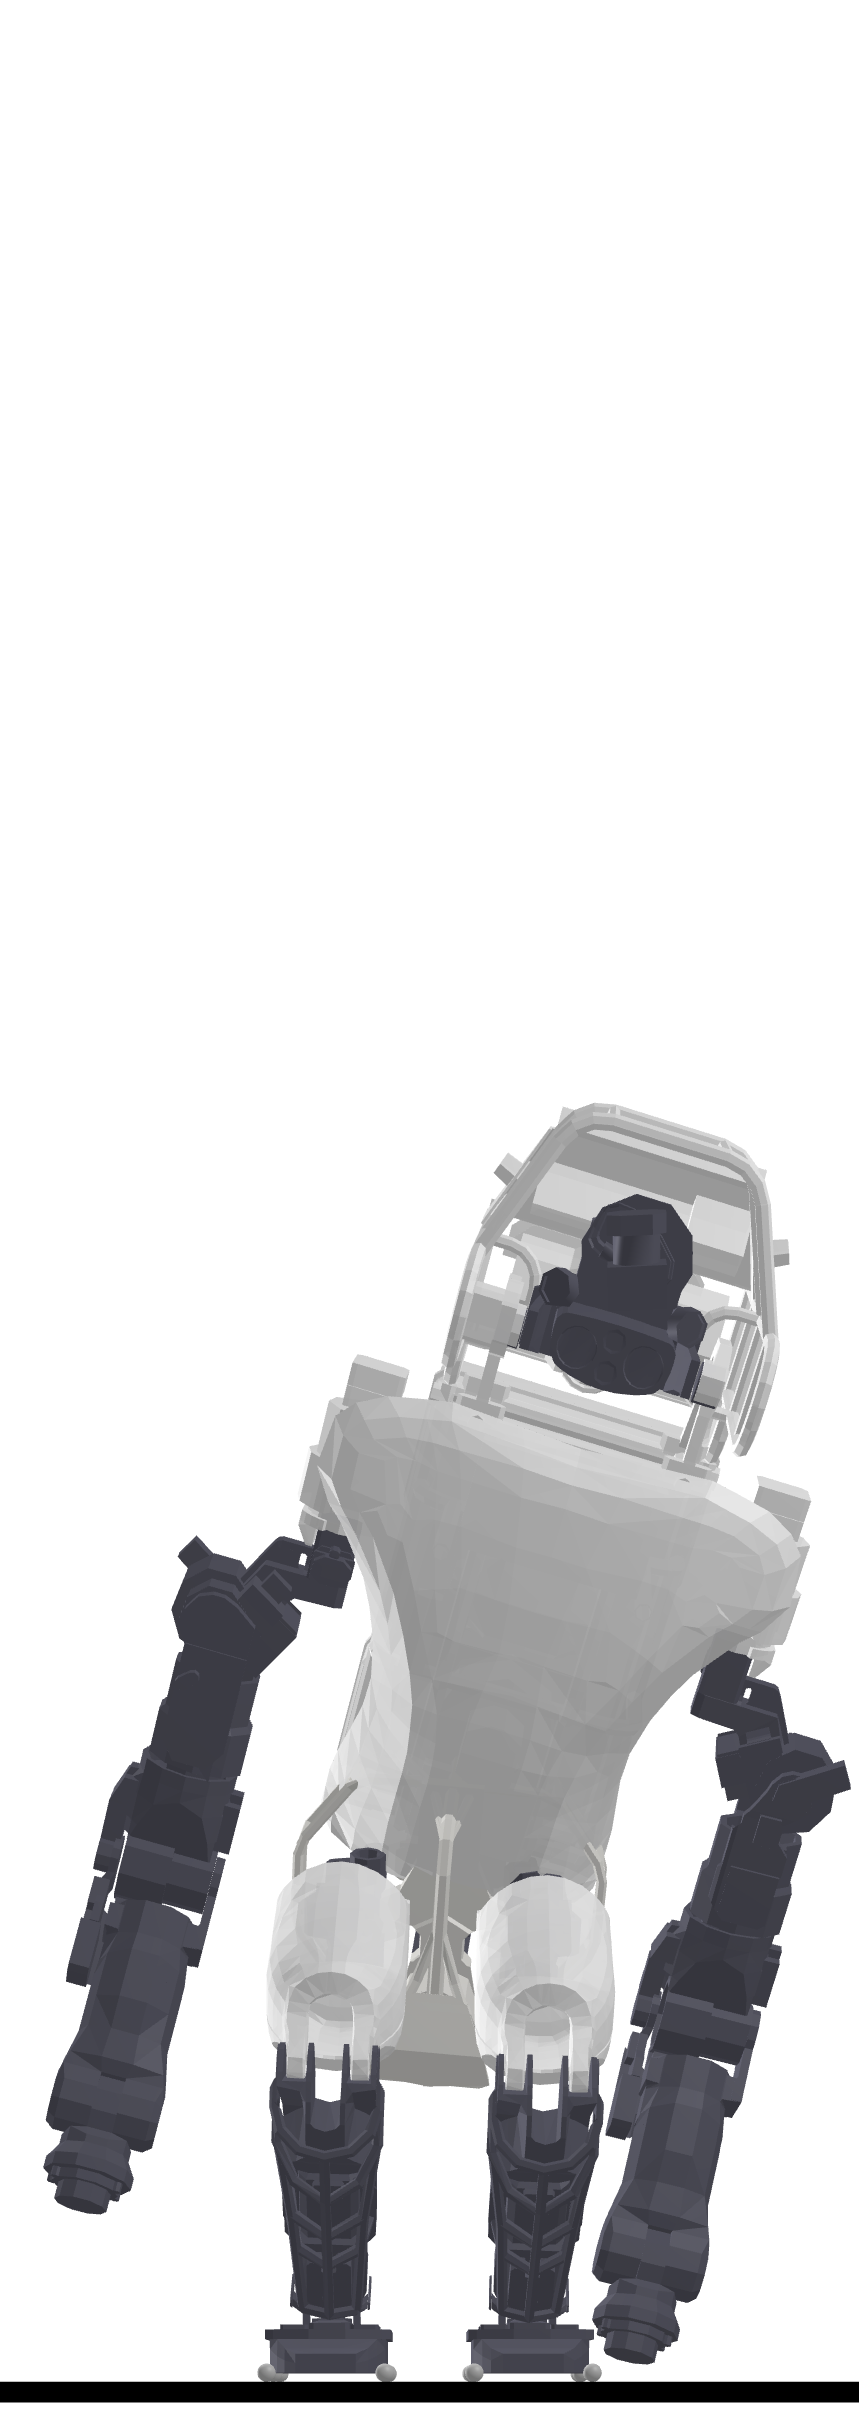
\includegraphics[height=5.0cm]{dojo/atlas4.png}
	\caption[Atlas drop test simulation]{Atlas drop simulation. Dojo simulates this system with 403 maximal-coordinates states, 30 joint constraints, 36 inputs, and 8 contact points in real-time at 65 Hz. Dojo respects floor-feet penetration constraints to machine precision, while MuJoCo suffers from centimeters of interpenetration and is unstable at low simulation rates.}
	\label{dojo_atlas_drop}
\end{figure}

A comparison with MuJoCo is performed measuring penetration violations with the floor for different simulation rates (Table \ref{dojo_contact_violation_results}).

\begin{table}[H]
	\centering
	\caption[Contact violation comparison between Dojo and MuJoCo for Atlas drop test]{Contact violation for Atlas drop. Comparison between Dojo and MuJoCo for foot contact penetration  (millimeters) with the floor for different time steps (seconds). Dojo strictly enforces no penetration. When Atlas lands, its feet remains above the ground by an infinitesimal amount. In contrast, MuJoCo exhibits significant penetration through the floor (i.e., negative values).}
	\begin{tabular}{c c c c}
		\toprule
		\textbf{Time Step} & \textbf{0.1} & \textbf{0.01} & \textbf{0.001} \\
		\toprule
		MuJoCo & \mbox{failure} & \textminus 28 & \textminus 46 \\
		Dojo & \textbf{+1e{-}12} & \textbf{+1e{-}7} & \textbf{+8e{-}6} \\
		\toprule
	\end{tabular}
	\label{dojo_contact_violation_results}
\end{table}

\paragraph{Friction-cone comparison.}
The effect of friction-cone approximation is demonstrated by simulating a box that is initialized with lateral velocity before impacting and sliding along a flat surface. For a pyramidal approximation, in the probable scenario where its vertices are not aligned with the direction of motion, velocity drift occurs for a linearized cone implemented in Dojo and MuJoCo (Fig. \ref{dojo_velocity_drift}). 

\begin{figure}[H]
	\begin{center}
		\begin{tikzpicture}
			\draw (0, 0) node[inner sep=0] {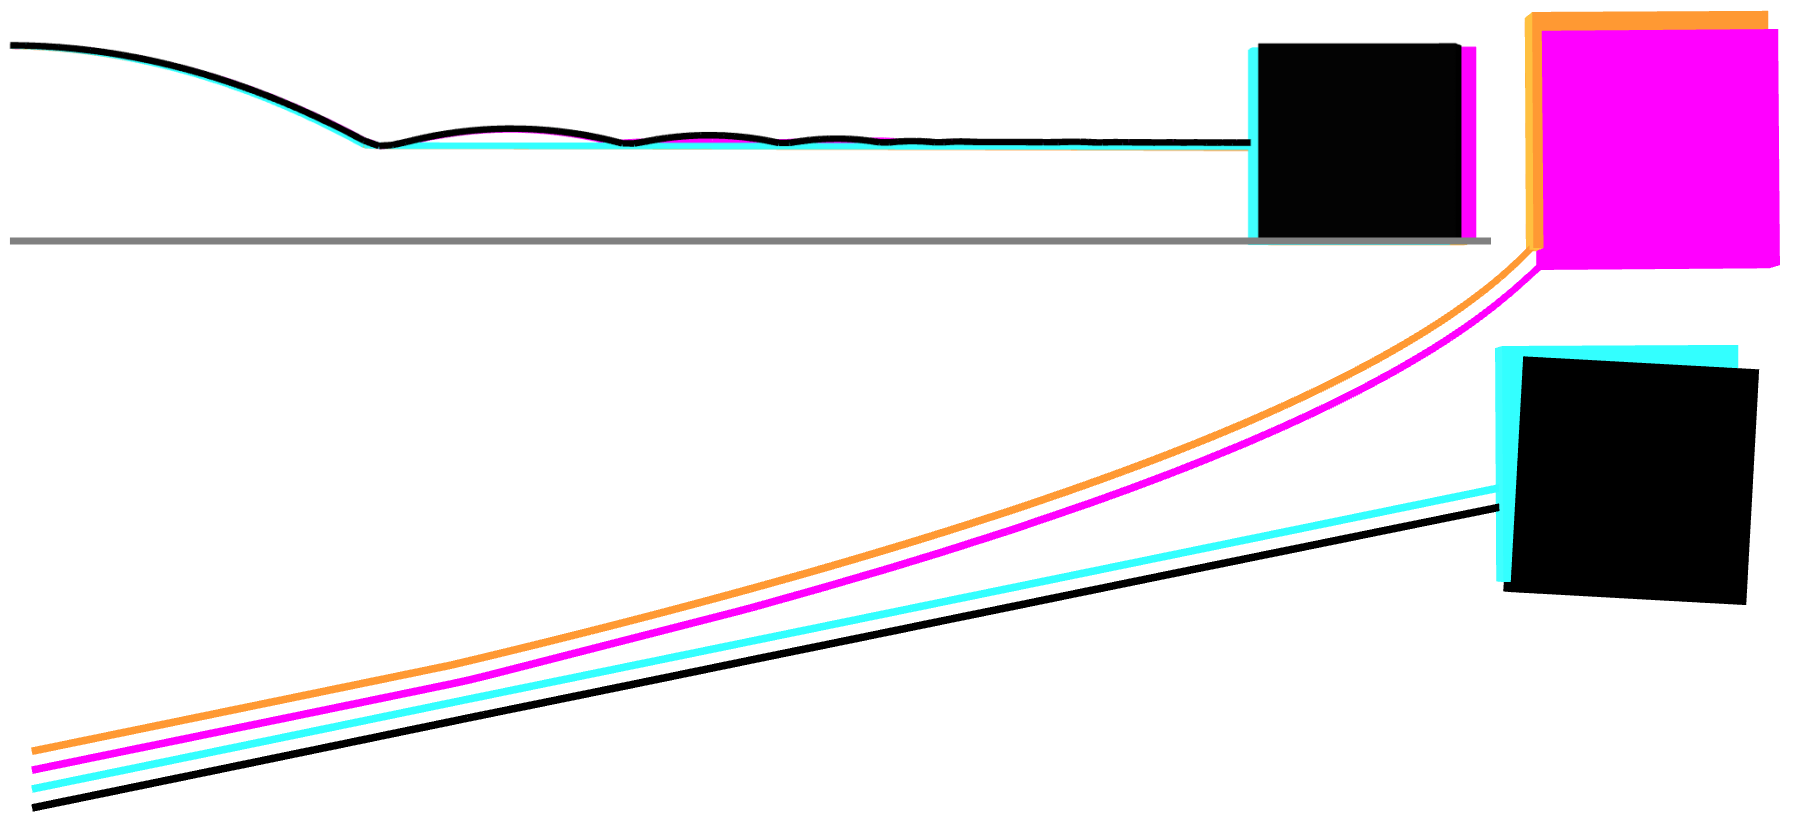
\includegraphics[width=0.5\linewidth]{dojo/cone_compare_final.png}};
			\draw (+0.0, +1.7) node {side view};
			\draw (+0.0, -1.4) node {top view};
		\end{tikzpicture}
	\end{center}
	\caption[Velocity drift comparison between linearized and second-order friction cones]{Velocity drift resulting from friction-cone approximation. Comparison between a box sliding with approximate cones having four vertices implemented in MuJoCo (magenta) and Dojo (orange) versus MuJoCo's (black) and Dojo's (blue) nonlinear friction cones. Dojo's nonlinear friction cone gives the physically correct straight line motion, while linear friction-cone approximations lead to lateral drift. MuJoCo's nonlinear friction cone exhibits a minor rotational drift.}
	\label{dojo_velocity_drift}
\end{figure}

The complementarity problem with $P$ contact points requires $2 P (1 + 2 d)$ decision variables for contact and a corresponding number of constraints, where $d$ is the degree of parameterization (e.g., double parameterization: $d=2$). While it is possible to reduce such artifacts by increasing the number of vertices in the approximation of the second-order cone, this increases the computational complexity. Such approximation is unnecessary in Dojo as we handle the exact nonlinear cone constraint efficiently and reliably with optimization tools from cone programming; the result is accurate sliding.

\paragraph{Energy and momentum conservation.}

An accurate physics engine conserves important physical quantities like energy and momentum. Following the methodology from \cite{erez2015simulation}, we simulate ``astronaut,'' a free-floating humanoid, and measure the drift of these quantities (Fig. \ref{dojo_drift}). 

\begin{figure}[H]
	\centering
	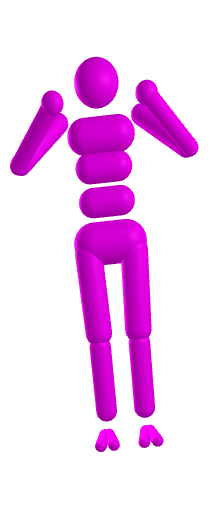
\includegraphics[height=3.8cm]{dojo/astronaut1.png} 
	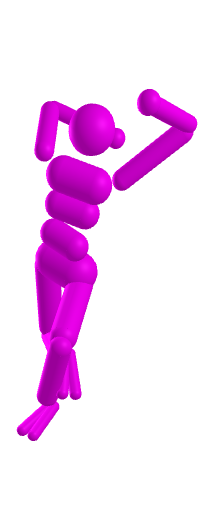
\includegraphics[height=3.8cm]{dojo/astronaut2.png}
	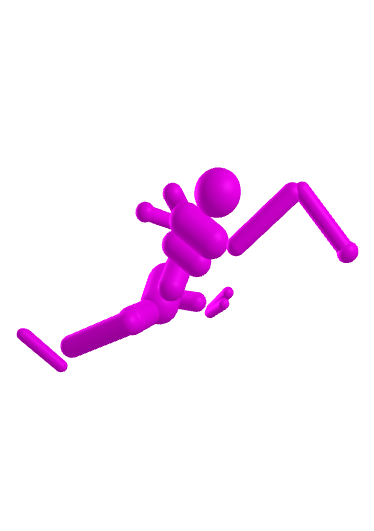
\includegraphics[height=3.8cm]{dojo/astronaut3.png}
	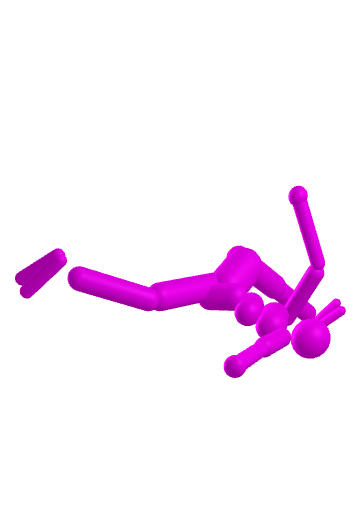
\includegraphics[height=3.8cm]{dojo/astronaut4.png}
	\caption[Astronaut energy and momentum drift simulation]{Astronaut simulation for energy and momentum conservation test. Joints are initialized with zero velocities and randomly actuated for 1 second. The simulation is visualized, from left to right.}
	\label{dojo_astronaut}
\end{figure}

There is no internal damping or springs, joint limits, or contact, and gravity is turned off. The astronaut is initialized with no linear or angular velocity and momentum drift is computed after one second of uniformly sampled actuation: $u \sim \mathcal{U}(0,0.05)$. Energy drift is computed over a 100 second period after 1 second of random actuation. MuJoCo exhibits drift in all scenarios. Characteristic of its variational integrator, Dojo conserves both linear and angular momentum to machine precision. Energy does not drift for Dojo but exhibits small bounded oscillations that decrease in amplitude as the time step decreases (Fig. \ref{dojo_drift}). Conservation of energy to machine precision with variational integrators is possible and is a topic of current research \cite{sharma2018energy}.

\begin{figure}[H]
	\begin{center}
		\includegraphics[width=0.4\columnwidth, height=6.0cm]{dojo/astronaut_energy.tikz}
		\includegraphics[width=0.5\columnwidth, height=6.0cm]{dojo/astronaut_momentum_freq.tikz}
	\end{center}
	\caption[Astronaut energy and momentum drift numerical comparison between Dojo and MuJoCo]{
		Energy and momentum conservation comparison between MuJoCo and Dojo for the astronaut simulation (Fig \ref{dojo_astronaut}) using time steps ranging from 0.001 to 0.1 second. Momentum drift is measured after actuating the astronaut for 1 second with random controls. Energy drift is measured over a 100 second simulation after 1 second of random actuation.}
	\label{dojo_drift}
\end{figure}

\subsection{Planning} 

Iterative LQR \cite{howell2022trajectory} utilizes implicit gradients from Dojo to perform trajectory optimization on three systems: planar box, hopper, and quadruped. A comparison is performed with MuJoCo and finite-difference gradients. The results for the quadruped are visualized in Fig. \ref{dojo_trajopt_vis} and all tested systems are summarized in Table \ref{dojo_trajopt_results}. 

\begin{figure}[H]
	\centering
	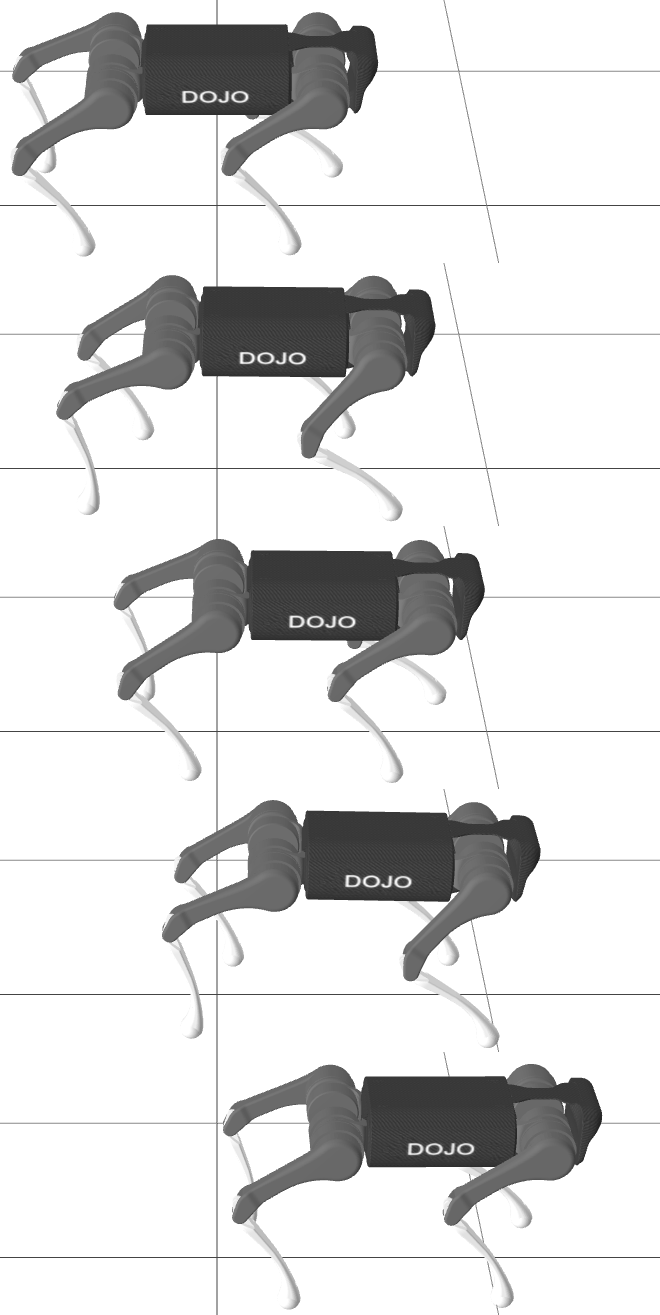
\includegraphics[width=0.25\textwidth]{dojo/quadruped_stack.png}
	\caption[Locomotion plan for quadruped]{Locomotion plan for quadruped generated using trajectory optimization. Time progresses top to bottom.}
	\label{dojo_trajopt_vis}
\end{figure}

\paragraph{Box.} Inputs are optimized to move a stationary rigid body that is resting on a flat surface (Fig. \ref{dojo_gradient_compare}) to a goal location that is either to the right or up in the air $1$ meter. The planning horizon is $1$ second and the controls are initialized with zeros. Dojo uses a time step $h = 0.1$, whereas MuJoCo uses $h = 0.01$ to prevent significant contact violations with the floor. MuJoCo fails in the scenario with the goal in the air, while Dojo succeeds at both tasks.

\paragraph{Hopper.} The hopping robot \cite{raibert1989dynamically} with $m = 3$ controls and $n = 14$ degrees-of-freedom is tasked with moving to a target pose over $1$ second. Similar, although not identical, models and costs are used. Dojo uses a time step $h = 0.05$ whereas MuJoCo uses $h = 0.01$. The hopper is initialized with controls that maintain its standing configuration. Quadratic costs are used to penalize control effort and cost shaping is utilized to set target positions in the air and the goal pose. The optimizer typically finds a single-hop motion.

\paragraph{Quadruped.} The torque-controlled Unitree A1 quadruped \cite{unitree2022a1} with $m = 12$ controls and $n = 36$ degrees-of-freedom is tasked with moving to a goal location over a planning horizon $T = 41$ with time step $h = 0.05$. Controls are initialized to compensate for gravity and there are costs on tracking a target kinematic gait and control inputs. The optimizer finds a dynamically feasible motion that closely tracks the kinematic plan.

\begin{table}[H]
	\centering
	\caption[Numerical planning results for box, hopper, and quadruped]{Planning results. Comparison of final cost value, goal constraint violation, and total number of iterations for a collection of systems with maximal (max) and minimal (min) representations, optimized with iterative LQR \cite{li2004iterative} using Dojo with implicit gradients or MuJoCo (M) with finite-difference gradients.}
	\begin{tabular}{c c c c}
		\toprule
		\textbf{System} & \textbf{Cost} & \textbf{Violation} & \textbf{Iterations}\\
		\toprule
		box right (max) & 14.5 & 3e{-}3 & \textbf{30} \\
		box right (M) & \textbf{13.5} & \textbf{3e{-}3} & 95 \\
		\hline
		box up (max) & \textbf{14.5} & \textbf{3e{-}3} & \textbf{106} \\
		box up (M) & \mbox{failure} & 1.0 & -\\
		\hline
		hopper (max) & 10.2 & 4e{-}3 & \textbf{57} \\
		hopper (min) & \textbf{8.9} & \textbf{1e{-}3} & 96 \\
		hopper (M) & 26.7 & 2e{-}3 & 66 \\
		\hline
		quadruped (min) & 2e{-}2 & 3e{-}4 & 20 \\
		\toprule
	\end{tabular}
	\label{dojo_trajopt_results}
\end{table}

In the examples, gradients are computed with $\kappa = 3e{-}4$. Overall, we find that final results from both engines are similar. However, importantly, MuJoCo is enforcing soft contact whereas Dojo simulates hard contact. Further, MuJoCo requires a time step $h = 0.01$ for stable simulation, whereas Dojo works well with $h = 0.05$. 

\subsection{Policy optimization}

Gym-like environments \cite{brockman2016openai, duan2016benchmarking}: ant and half-cheetah are implemented in Dojo and we train static linear policies for locomotion. As a baseline, we employ Augmented Random Search (ARS) \cite{mania2018simple}, a gradient-free approach coupling random search with a number of simple heuristics. For comparison, we train the same policies using augmented gradient search (AGS) which replaces the stochastic-gradient estimation of ARS with the Dojo's implicit gradients. Policy rollouts are visualized in Fig. \ref{dojo_rl_vis} and results are summarized in Table \ref{dojo_rl_results}.

\begin{figure}[H]
	\begin{center}
		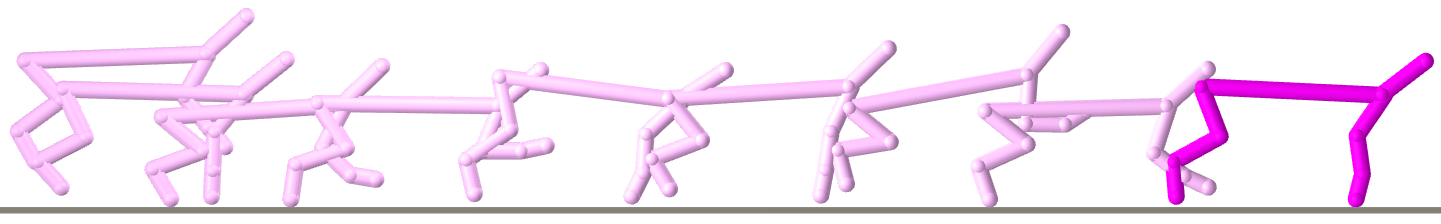
\includegraphics[width=0.5\columnwidth]{dojo/halfcheetah_ars.png}
		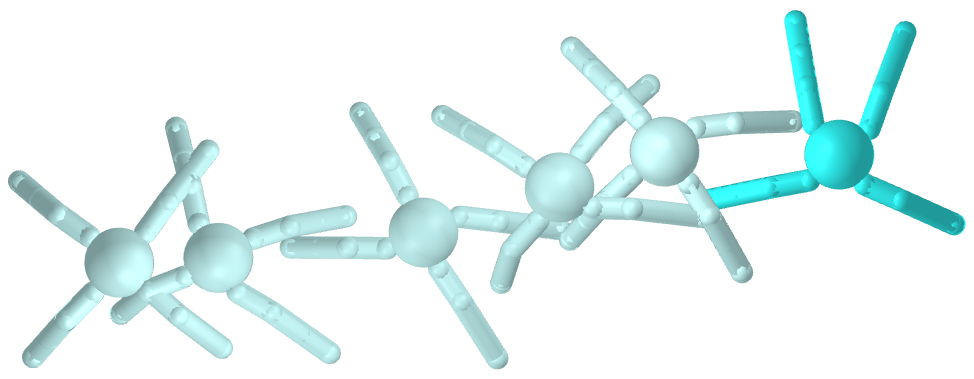
\includegraphics[width=0.5\columnwidth]{dojo/ant_ars.png}
	\end{center}
	\caption[Learned policy rollouts for half-cheetah and ant]{Learned policy rollouts for half-cheetah (top) and ant (bottom) generated using Augmented Random Search. Time progresses left to right.}
	\label{dojo_rl_vis}
\end{figure}

\paragraph{Half-cheetah.}
This planar system \cite{brockman2016openai} with $m = 6$ controls and $n = 18$ degrees-of-freedom is rewarded for forward velocity and penalized for control effort over a horizon $T = 80$ with time step $h = 0.05$. 

\paragraph{Ant.}
The system \cite{brockman2016openai} has $m = 8$ controls and $n = 28$ degrees-of-freedom and is rewarded for forward motion and staying alive and is penalized for control effort and contact over a horizon $T = 150$ with time step $h = 0.05$.

\begin{table}[H]
	\centering
	\caption[Numerical policy optimization results for half-cheetah and ant]{Policy optimization results. Comparison of total reward, number of simulation-step and gradient evaluations for policies trained with Augmented Random Search (ARS) \cite{mania2018simple} and Augmented Gradient Search (AGS). The results are averaged over the best 3 out of 5 runs with different random seeds.} 
	\begin{tabular}{c c c c}
		\toprule
		\textbf{System} & \textbf{Reward} & \textbf{Simulation} & \textbf{Gradient} \\
		\toprule
		half-cheetah (ARS) & 46 $\pm$ 24 & 3e{+}4 & 0 \\
		ant (ARS)          & 64 $\pm$ 15 & 2e{+}5 & 0 \\
		half-cheetah (AGS) & 44 $\pm$ 24 & \textbf{5e{+}3} & 5e{+}3 \\ 
		ant (AGS)          & 54 $\pm$ 28 & \textbf{2e{+}4} & 2e{+}4 \\
		\toprule
	\end{tabular}
	\label{dojo_rl_results}
\end{table}

First, we are able to successfully train policies using this simple learning algorithm in Dojo's hard contact environments. Second, MuJoCo requires smaller $h = 0.01$ time steps for stable simulation, whereas Dojo is stable with $h = 0.05$. Third, our initial experiments indicate that it is possible to utilize Dojo's implicit gradients for more efficient training compared to the derivative-free approach.

\subsection{System identification} 

System identification is performed on an existing real-world dataset of trajectories collected by throwing a box on a table with different initial conditions \cite{pfrommer2021contactnets}. We learn a set of parameters $\theta = (\mu, p^{(1)}, \dots, p^{(8)})$ that include the friction coefficient $\mu$, and 3-dimensional vectors $p^{(i)}$ that represent the position of vertex $i$ of the box with respect to its center of mass.

Each trajectory is decomposed into $T-2$ triplets of consecutive configurations: $Z = (z_{-}, z, z_{+})$, where $T$ is the number of time steps in the trajectory. Using the initial conditions $z_{-}, z$ from a tuple, and an estimate of the system's parameters $\theta$, Dojo performs one-step simulation to predict the next state, $\hat{z}_{+}$. Implicit gradients are utilized by a Gauss-Newton method to learn the system parameters.

\begin{figure}[t]
	\begin{center}
		\begin{tikzpicture}
			\draw (0, 0) node[inner sep=0] {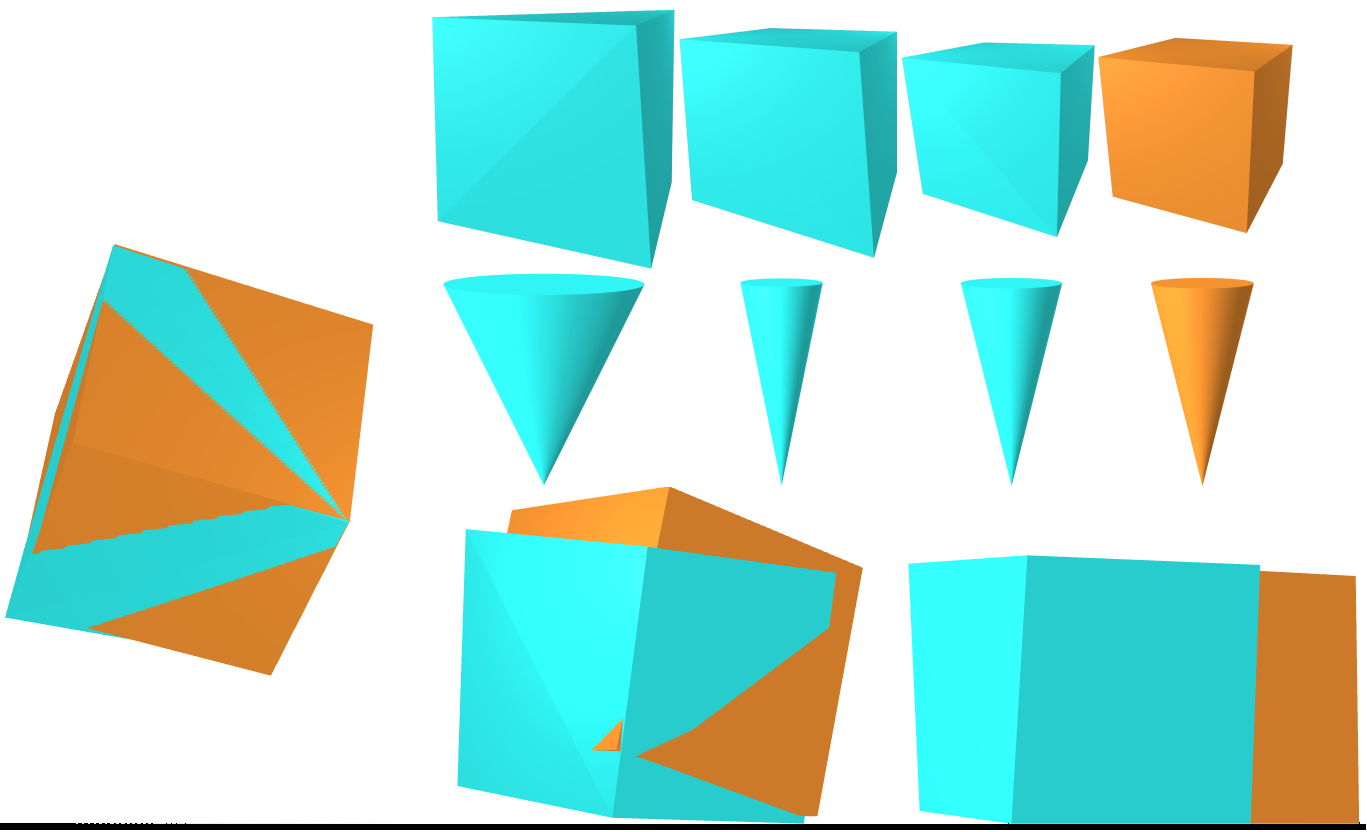
\includegraphics[width=0.5\linewidth]{dojo/box_and_cone_and_toss.png}};
			\draw (-0.7, +2.9) node {(1)};
			\draw (+0.6, +2.9) node {(5)};
			\draw (+1.8, +2.9) node {(50)};
			\draw (+2.95, +2.9) node {(truth)};
		\end{tikzpicture}
	\end{center}
	
	\caption[Learned friction parameters and contact geometry for box (top). Real-to-sim simulation for learned box parameters (bottom)]{System identification. Top right: Learning box geometry and friction cone to less than $5\%$ error. Bottom: Simulated trajectory of the box using the learned properties (blue) compared to ground truth (orange).}
	\label{dojo_real2sim}
\end{figure}

The parameters are learned by minimizing the following loss: 
\begin{align}
	\mathcal{L}(\mathcal{D}, \theta) = \sum_{Z \in \mathcal{D}} L(Z, \theta) = \sum_{Z \in \mathcal{D}} \frac{1}{2} ||\mbox{\textbf{Dojo}}(z_{-}, z; \theta) - z_{+}||_W^2,
\end{align}
where $||\cdot||_W$ is a weighted norm, which aims to minimize the difference between the ground-truth trajectories and physics-engine predictions. We use gradients:
\begin{equation}
	\frac{\partial L}{\partial \theta} = {\frac{\partial \mbox{\textbf{Dojo}}}{\partial \theta}}^T W \left(\mbox{\textbf{Dojo}}(z_{-}, z; \theta) - z_{+} \right),
\end{equation}
and approximate Hessians: 
\begin{align}
	\frac{\partial^2 L}{\partial \theta^2} &\approx {\frac{\partial \mbox{\textbf{Dojo}}}{\partial \theta}}^T W \frac{\partial \mbox{\textbf{Dojo}}}{\partial \theta}.
\end{align}
Gradients are computed with $\kappa = 3e{-}4$.

After training, the learn parameters are within $5\%$ of the geometry and best-fit friction coefficient for the box from the dataset. We complete the transfer from real-to-sim and simulate the learned system parameters in Dojo, comparing it to the ground-truth dataset trajectories. Results are visualized in Fig. \ref{dojo_real2sim}.

\section{Limitations} \label{dojo_limitations}

The computation cost of Dojo per simulation step is greater than many existing engines. The greater computational complexity enables superior simulation accuracy at the cost of increased wall-clock time and is a trade-off that must be considered by the user for a particular application. Additionally, because Dojo solves a nonlinear complementarity problem (i.e, non-convex problem) at each time step the engine provides no guarantees of converging to a solution. In practice, we do no find this to be a problem, but for time- or safety-critical applications this should be a consideration. Further, it remains to be seen how well sim-to-real transfer works, in comparison to existing engines, particularly for manipulation tasks with a large number of contact interactions.

\section{Future work} \label{dojo_future_work}

Dojo is designed from physics- and optimization-first principles to enable better gradient-based optimization for motion planning, control, reinforcement learning, and system identification. The engine makes several advancements over previous state-of-the-art engines for robotics: First, the variational integrator enables stable simulation at low sample rates. Second, the contact model includes an improved friction model that eliminates artifacts like creep, particularly for sliding, and hard contact for impact is achieved to machine precision. This should enable superior sim-to-real transfer for both locomotion and manipulation applications. The underlying interior-point solver, developed specifically for solving NCPs, is numerically robust and requires practically no hyperparameter tuning for good performance across numerous systems, and handles cone and quaternion variables. Third, the engine efficiently returns implicit gradients that are smooth and analytical, providing useful information through contact events. Fourth, in addition to building and providing an open-source tool, the physics and optimization algorithms presented can improve many existing engines.

In terms of features, reliability, and wall-clock time, MuJoCo--the product of a decade of excellent software engineering--is impressive. As development of Dojo continues, we expect to make significant progress in all of these areas. However, fundamentally, Dojo's approach of solving an NCP with a primal-dual interior-point method will likely be computationally more expensive compared to MuJoCo's convex soft-contact model, which can never entirely recover accurate solutions even at higher sampling frequencies. This is the fundamental trade-off Dojo makes for robotics applications: greater computational cost for accurate physics and smooth gradients.

A number of future improvements to Dojo are planned. First, Dojo currently implements simple collision detection (e.g., sphere-halfspace, sphere-sphere). Natural extensions include support for convex primitives and curved surfaces. Another improvement is adaptive time stepping. Similar to advanced numerical integrators for stiff systems, Dojo should take large time steps when possible and adaptively modify the time step in cases of numerical difficulties or physical inaccuracies. Finally, hardware-accelerator support for Dojo would potentially enable faster simulation and optimization.

Perhaps the most important remaining question is whether the physics and optimization improvements from this work translate into better transfer of simulation results to successes on real-world robotic hardware. In this thrust, future work will explore the transfer of control policies trained in Dojo to hardware and deployment of the engine in model predictive control frameworks.

In conclusion, we have presented a new physics engine, Dojo, specifically designed for robotics. This tool is the culmination of a number of improvements to the contact dynamics model and underlying optimization routines, aiming to advance state-of-the-art physics engines for robotics by improving physical accuracy and differentiability. 

\section*{Acknowledgments}
The authors would like to thank Jan Br{\"u}digam for  \texttt{ConstrainedDynamics.jl}, an open-source library which served as a foundation for Dojo's maximal-coordinates state representation, as well as early technical discussions and support; and Suvansh Sanjeev for assistance with the Python interface. Toyota Research Institute provided funds to support this work. 

\section{Appendix: Quaternion Algebra}
\label{dojo_quaternion_algebra}
In this section we introduce a set of conventions for notating standard quaternion operations, adopted from \cite{brudigam2020linear,jackson2021planning}, and employed in the rotational part of our variational integrator \eqref{dojo_rotational_integrator}.

Quaternions are written as four-dimensional vectors:
\begin{equation}
	q = (s, v) = (s, v_1, v_2, v_3) \in \mathbf{H},
\end{equation}
where $s$ and $v$ are scalar and vector components, respectively. Dojo employs unit quaternions (i.e., $q^T q = 1$) to represent orientation, providing a mapping from the local body frame to a global inertial frame.

Quaternion multiplication is represented using linear algebra (i.e., matrix-vector and matrix-matrix products). Left and right quaternion multiplication, 
\begin{equation} 
	q^a \otimes q^b 
	= \begin{bmatrix}
		s^a s^b - (v^a)^T v^b \\
		s^a v^b + s^b v^a + v^a \times v^b
	\end{bmatrix} 
	= L(q^a)q^b = R(q^b) q^a ,
\end{equation}
where $\times$ is the standard vector cross product, is represented using the matrices:
\begin{align}
	L(q) &= \begin{bmatrix}
		s & -v^T \\
		v & s I_3 + \mathbf{skew}(v)
	\end{bmatrix} \in \mathbf{R}^{4 \times 4},\\
	R(q) &= \begin{bmatrix}
		s & -v^T \\
		v & s I_3 - \mathbf{skew}(v)
	\end{bmatrix} \in \mathbf{R}^{4 \times 4},
\end{align}

where, 
\begin{equation}
	\mathbf{skew}(x) = \begin{bmatrix}  
		0 & -x_3 & x_2 \\
		x_3 & 0 & -x_1 \\
		-x_2 & x_1 & 0 
	\end{bmatrix},
\end{equation}
is defined such that,
\begin{equation}
	\mathbf{skew}(x) y = x \times y ,
\end{equation}
and $I_3$ is a 3-dimensional identity matrix. The vector component of a quaternion, 
\begin{equation} 
	v = V q,
\end{equation}
is extracted using the matrix:
\begin{equation}
	V = \begin{bmatrix}
		\mathbf{0} & I_3
	\end{bmatrix} \in \mathbf{R}^{3 \times 4},
\end{equation}
and quaternion conjugate: 
\begin{equation} 
	q^{\dagger} = \begin{bmatrix} s \\ -v \end{bmatrix} = T q,
\end{equation}
is computed using:
\begin{equation}
	T = \begin{bmatrix}
		1 & \mathbf{0}^T \\
		\mathbf{0} & -I_3
	\end{bmatrix} \in \mathbf{R}^{4 \times 4}.
\end{equation}
	

